\subsection*{ГЛ12 1}
\begin{figure}[h]
	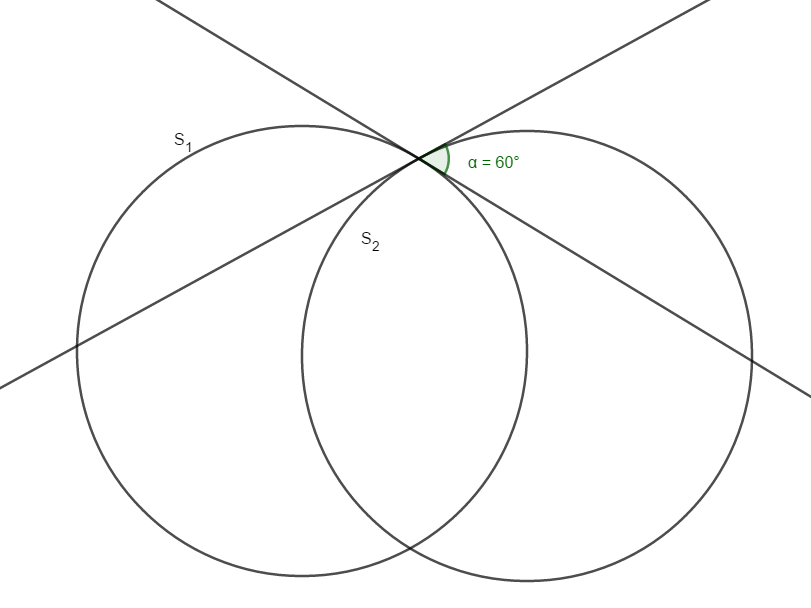
\includegraphics[width=0.75\linewidth]{pic3}
\end{figure}
Пусть P -- заданная точка, тогда проведем через неё любые 2 несовпадающие прямые, пересекающие конику в 2 точках каждая. Назовем эти точки $A_1, A_2, A_3, A_4$ и проведем прямые $A_1A_3, A_2A_4, A_1A_2, A_3A_4$. Пусть $K = A_1A_3 \cap A_2A_4$ и $L = A_1A_2 \cap A_3A_4$, проведем прямую $KL$, тогда прямые $PN$ и $PM$ будут касательными.
		